\section{\large Estado del Arte}  

\subsection{Blockchain para Registros Gubernamentales y Gestión de Sanciones} 

La aplicación de la tecnología Blockchain y DLT (Distributed Ledger Technology) en la administración pública ha sido un área de creciente interés, impulsada por las promesas teóricas de Inmutabilidad, Transparencia y Auditoría mejorada, fundamentales para la Confianza Descentralizada. La investigación sugiere que Blockchain puede transformar la gestión de registros oficiales, como licencias, títulos de propiedad y, potencialmente, multas o sanciones como los fotocomparendos. 

\paragraph{Análisis de Aplicación}
La capacidad de crear un registro de Transacciones criptográficamente asegurado y distribuido permite generar una pista de auditoría fiable y resistente a la manipulación. Cada registro de sanción, incluyendo sus Metadatos (fecha, hora, ubicación, tipo de infracción) y el Hash de la evidencia asociada, puede ser anclado a la cadena, proporcionando una fuente única de verdad verificable por las partes autorizadas. Esto se alinea con los principios de Sistemas Distribuidos aplicados a la gobernanza. 

\paragraph{Blockchains Públicas vs. Permisionadas}
En el contexto gubernamental, la literatura y los estudios piloto tienden a favorecer las blockchains permisionadas (o de consorcio). Si bien las blockchains públicas ofrecen máxima transparencia, las permisionadas permiten a las entidades gubernamentales controlar quién puede participar en la red (validar transacciones, acceder a datos), gestionar mejor la privacidad (crucial para datos ciudadanos) y, a menudo, ofrecer mayor rendimiento y escalabilidad. La elección impacta directamente en el modelo de Confianza Descentralizada implementado. 

\paragraph{Madurez y Barreras}
Aunque existen numerosos estudios y proyectos piloto (ej., registros de tierras en Suecia o Georgia, identidad digital en Estonia), las implementaciones a gran escala para la gestión integral de sanciones administrativas aún son limitadas. La madurez es variable. Las barreras reconocidas incluyen la complejidad técnica, la necesidad de marcos legales y regulatorios adaptados, la interoperabilidad con sistemas heredados, los costos iniciales de implementación y la adopción tanto por parte de las instituciones como de los ciudadanos. La Percepción Pública de la Tecnología Blockchain también juega un rol significativo. 

\subsection{Integración de Blockchain e IPFS para Datos Voluminosos y Verificables} 

El almacenamiento directo de datos voluminosos (como imágenes o vídeos de alta resolución) en una Blockchain es ineficiente y costoso. La literatura técnica y diversos prototipos exploran la integración de Blockchain con sistemas de Almacenamiento Direccionable por Contenido como IPFS (InterPlanetary File System) para abordar este desafío. 

\paragraph{Estado Actual} El enfoque predominante consiste en almacenar el dato voluminoso (la imagen del fotocomparendo) en IPFS, obteniendo un Hash único basado en su contenido. Este Hash IPFS, junto con otros Metadatos relevantes, se almacena en una Transacción Blockchain. Este modelo aprovecha la eficiencia de IPFS para el almacenamiento distribuido y la fortaleza de Blockchain para el registro inmutable y verificable del puntero (el Hash) y los metadatos asociados. 

\paragraph{Ventajas y Desafíos} Las ventajas logradas incluyen la verificabilidad (cualquier cambio en el archivo IPFS cambiaría su hash, invalidando el enlace en la Blockchain), la resiliencia potencial (si múltiples nodos almacenan el archivo) y el direccionamiento por contenido inherente a IPFS. Sin embargo, persisten desafíos persistentes significativos: 

\paragraph{Persistencia de Datos (Pinning)} Los datos en IPFS solo persisten mientras algún nodo los esté "pineando" (almacenando activamente). Garantizar la persistencia a largo plazo de la evidencia requiere mecanismos o servicios de pinning fiables, que pueden tener costos asociados. 

\paragraph{Disponibilidad} La recuperación del archivo depende de que los nodos que lo almacenan estén en línea y accesibles. 

\paragraph{Costos a Largo Plazo} El almacenamiento distribuido no es necesariamente gratuito, especialmente si se requieren garantías de disponibilidad y persistencia. 

\paragraph{Gestión de la Privacidad} Los datos en IPFS son típicamente accesibles públicamente si se conoce el hash. Para evidencia sensible, se requerirían capas adicionales de encriptación antes de la subida a IPFS, añadiendo complejidad. 

\subsection{Gestión de Evidencia Digital y Cadena de Custodia con DLT}

La integridad y la cadena de custodia de la evidencia digital son cruciales en procesos sancionatorios. Blockchain/DLT ofrece mecanismos basados en Criptografía Aplicada para fortalecer estos aspectos. 

\paragraph{Fortalecimiento de la Integridad y Trazabilidad} Al registrar el Hash de la evidencia digital (imagen del fotocomparendo) en una Transacción Blockchain, se crea un sello de tiempo (timestamping) inmutable y verificable. Cualquier intento posterior de modificar la evidencia original resultaría en un hash diferente, lo que permitiría detectar fácilmente la manipulación. La secuencia de transacciones en la Blockchain proporciona una trazabilidad auditable del ciclo de vida de la evidencia (captura, registro). 

\paragraph{Comparación y Valor Añadido} En comparación con los sistemas tradicionales (bases de datos centralizadas, logs de servidor), que pueden ser susceptibles a alteraciones internas o fallos únicos, la DLT aporta un valor añadido significativo al distribuir la confianza y hacer que la manipulación sea computacionalmente inviable (principio de Inmutabilidad). Esto refuerza la Confianza Descentralizada en la validez de la evidencia presentada, reduciendo potenciales disputas. 

\paragraph{Estándares Emergentes} En el ámbito de la tecnología blockchain, observamos la consolidación de estándares emergentes en diversas áreas, que representan un consenso práctico y técnico en ausencia de normas formales universalmente ratificadas. 

Un área clave es la Seguridad de Smart Contracts. Para construir confianza y fiabilidad en las aplicaciones descentralizadas (dApps) y mitigar vulnerabilidades, se están adoptando ampliamente prácticas que funcionan como estándares de facto: 
\begin{itemize}
    \item \textbf{Auditorías y Listas de Chequeo:} Metodologías promovidas por firmas especializadas como ConsenSys Diligence, Trail of Bits y OpenZeppelin se han vuelto habituales. 
    \item \textbf{Patrones de Diseño Seguro:} Se aplican convenciones como Checks-Effects-Interactions y el uso de proxies actualizables (UUPS, Transparent Proxy), aunque estos patrones continúan evolucionando. 
    \item \textbf{Estándares de Reporte de Vulnerabilidades:} Propuestas como las EIPs (Ethereum Improvement Proposals) relacionadas con la seguridad ayudan a estandarizar la comunicación de fallos.
\end{itemize}

Otra área fundamental donde emergen estándares es la Gestión de Evidencia Digital y Cadena de Custodia mediante Blockchain/DLT. Aunque todavía no existe una norma global única (como un estándar ISO específico para esta aplicación), sí se está formando un fuerte consenso técnico sobre los principios tecnológicos clave para asegurar la integridad y fiabilidad:

\begin{itemize}
    \item \textbf{Hashing Criptográfico:}El uso de funciones hash para generar una huella digital única e infalsificable de la evidencia (como el CID en IPFS) es la práctica estándar para garantizar la integridad y detectar manipulaciones \parencite{benet2014ipfs}. 
    \item \textbf{Timestamping Inmutable:} Registrar el hash de la evidencia y sus metadatos en una transacción blockchain proporciona una marca de tiempo segura e inalterable, estableciendo una prueba fehaciente del momento del registro \parencite{nakamoto2008bitcoin}. 
    \item \textbf{Registro en Ledger Distribuido (DLT):} Utilizar la DLT como el libro contable distribuido para estos registros es el mecanismo reconocido para lograr inmutabilidad, transparencia controlada y auditabilidad \parencite{swan2015blockchain}, superando las limitaciones de las bases de datos centralizadas.
\end{itemize}

\subsection{Funcionamiento de los Fotocomparendos en Bogotá: Mecanismos, Regulación e Impacto} 
El sistema de fotocomparendos en Bogotá (FENIX) representa un modelo tecnológico y regulatorio diseñado para mejorar la seguridad vial mediante la detección automatizada de infracciones de tránsito \parencite{mintransporte2023}. Basado en cámaras de fotodetección ubicadas en zonas autorizadas por el Ministerio de transporte, este sistema combina vigilancia electrónica, validación humana y marcos legales específicos para sancionar conductas de riesgo \parencite{supertransporte2021}. Desde su implementación, ha logrado reducir siniestros en puntos críticos, aunque enfrenta desafíos técnicos y jurídicos. A continuación, se detalla su operación, criterios de aplicación y marco legal que lo regula \parencite{mintransporte2023}.

\paragraph{Marco Legal y Regulatorio} La implementación de fotocomparendos en Bogotá se sustenta en la Ley 1843 de 2017 \parencite{ley1843} y su reglamentación mediante resoluciones como la Resolución 20203040011245 \parencite{resolucion11245}. Estos instrumentos establecen cuatro criterios para instalar cámaras: 

\begin{enumerate}
    \item \textbf{Siniestralidad:}Ubicación en zonas con alto índice de accidentes. 
    \item \textbf{Prevención:} Disuasión de conductas peligrosas. 
    \item \textbf{Movilidad: } Optimización del flujo vehicular.
        \item \textbf{Historial de infracciones:} Enfoque en corredores con recurrentes violaciones.
\end{enumerate}

Adicionalmente, las autoridades deben garantizar la visibilidad de los dispositivos, señalizando su presencia al menos 500 metros antes de su ubicación \parencite{ley1843}, y cumplir con planes de seguridad vial alineados con políticas distritales. La Secretaría Distrital de Movilidad (SDM) ha enfrentado cuestionamientos legales, como los señalados por la Personería en 2018 \parencite{sdm2023camaras}.

\paragraph{Proceso Operativo de los Fotocomparendos} La implementación de fotocomparendos en Bogotá se sustenta en la Ley 1843 de 2017 \parencite{ley1843} y su reglamentación mediante resoluciones como la Resolución 20203040011245

\paragraph{Proceso Operativo de los Fotocomparendos }
\paragraph{Detección y Captura de Infracciones }
Las cámaras de fotodetección en Bogotá se clasifican en dos tipos \parencite{supertransporte2021, mintransporte2023}: 

\begin{itemize}
    \item \textbf{Automáticas: }Monitorean velocidades, semáforos en rojo y restricciones como pico y placa.
    \item \textbf{Semiautomáticas:}Vigilan bloqueos de calzadas, paradas prohibidas y recolección irregular de pasajeros.
\end{itemize}

Estos dispositivos, instalados en corredores de alta accidentalidad como la Avenida NQS o la Calle 100, capturan imágenes o videos que incluyen matrícula, fecha, hora y ubicación GPS14. Por ejemplo, en 2025, un conductor que exceda el límite de 50 km/h en la Avenida Boyacá será registrado por cámaras previamente señalizadas. 

\paragraph{Validación y Notificación }
Una vez detectada una presunta infracción, las pruebas se envían a un centro de análisis de la SDM, donde agentes de tránsito verifican:

\begin{itemize}
    \item Legibilidad de la matrícula. 
    \item Contexto de la violación (ejemplo: si un semáforo en rojo fue respetado).
    \item Datos del vehículo en el RUNT (Registro Único Nacional de Tránsito).
\end{itemize}

Tras validar la infracción, se genera un comparendo electrónico notificado al propietario del vehículo mediante correo certificado o plataformas digitales. El plazo máximo para emitir la sanción es de 10 días hábiles desde la detección, seguido de 3 días para su notificación. Si el domicilio registrado está desactualizado, el infractor podría no recibir la notificación, lo que no exime el pago \parencite{ley1843}. 

\paragraph{Tecnología y Transparencia }
El sistema combina: 
\begin{itemize}
    \item \textbf{Cámaras de última generación: }Equipadas con sensores de velocidad Lidar y visión nocturna. 
    \item \textbf{Plataforma de análisis IA: }Algoritmos que descartan falsos positivos (ejemplo: ambulancias en emergencia). 
        \item \textbf{Integración con RUNT:}Verificación instantánea de documentos como SOAT o tarjeta de operación.
\end{itemize}

Los datos se almacenan en servidores con cifrado AES-256, accesibles solo para funcionarios autorizados mediante autenticación biométrica.

\paragraph{Problemas Operativos }
\begin{itemize}
    \item \textbf{Notificaciones fallidas: }Errores en direcciones del RUNT causan sanciones no recibidas, acumulando intereses moratorios. 
    \item \textbf{Latencia en validaciones:  }En horas pico, el volumen de infracciones puede retrasar procesamientos hasta 72 horas.
\end{itemize}

\paragraph{Cuestionamientos Legales }
En 2018, la Personería de Bogotá identificó que el 15\% de las cámaras operaban sin autorización ministerial durante un periodo de transición legal. La SDM rectificó esta situación en 2019, regularizando todos los dispositivos bajo la Resolución 20203040011245 de 2020 \parencite{secretaria_movilidad2023}. 

\subsection{Aplicaciones Específicas en Gestión de Tráfico e Infracciones} 

Al revisar las Aplicaciones de Blockchain en la Gestión de Tráfico, Infracciones y Fotocomparendos, se observa que, si bien hay discusiones teóricas \parencite{yousfi2022its}, propuestas conceptuales \parencite{chen2024blockchain} y hasta una joven PYME española, las implementaciones prácticas que integren el flujo completo descrito en el prototipo (captura -> IPFS -> Blockchain -> Verificación -> Pago Automatizado con Billetera Digital) son escasas y se encuentran en fase de propuesta o son parciales \parencite{omar2024srtm,choquevilca2024blockchain}. 

\paragraph{Análisis de Existencia}
La literatura existente se centra más en componentes aislados \parencite{yousfi2022its}, uso de blockchain para registros vehiculares \parencite{ManiJosephP2023SmartAS}, seguros \parencite{dutta2023solution}, o gestión genérica de multas \parencite{omar2024srtm}, pero raramente combinando el almacenamiento de evidencia en IPFS con la automatización del pago vía billetera digital específicamente para fotocomparendos.

\paragraph{Arquitecturas y Resultados} Dada la escasez de implementaciones completas reportadas \parencite{AnandSingh_ProjectReport_Year,juit2024traffic}, es difícil generalizar sobre arquitecturas dominantes o resultados concretos para este caso de uso tan específico. Los estudios existentes a menudo se limitan a explorar la viabilidad teórica o a implementar módulos parciales \parencite{choquevilca2024blockchain}.

\paragraph{Lecciones Aprendidas:} La principal lección aprendida de áreas adyacentes es la importancia de abordar no solo los desafíos técnicos (Zheng et al., 2018) sino también los regulatorios, de gobernanza y de adopción (Tan et al., 2022). La ausencia de soluciones integrales reportadas para el flujo completo de gestión de fotocomparendos representa una brecha significativa en la aplicación práctica de estas tecnologías combinadas.

El análisis del estado del arte revela avances significativos, pero también limitaciones claras: 
  

\subsection{Avances Significativos} 

La tecnología Blockchain ha demostrado su potencial para crear registros gubernamentales más inmutables, transparentes y auditables. (Balcerzak et al., 2022; Meroni et al., 2023) 

La integración Blockchain + IPFS es una solución técnicamente viable y reconocida para gestionar datos voluminosos referenciados desde una cadena de bloques, mejorando la verificabilidad (Adel et al., 2023; Mishra et al., 2024). 

DLT ofrece mejoras sustanciales para la integridad y trazabilidad de la evidencia digital (Thanasas et al., 2025). 

Existen mecanismos (billeteras digitales, smart contracts, stablecoins) para habilitar pagos digitales automatizados en ecosistemas blockchain \parencite{antonopoulos2023mastering}.

\subsection{Limitaciones Identificadas} 
\paragraph{Madurez e Integración:}
Muchas aplicaciones gubernamentales de Blockchain son pilotos aislados (Zheng et al., 2018; Li et al., 2021). Falta integración entre sistemas y con procesos completos. 

\paragraph{Desafíos Técnicos: }
La persistencia y gestión a largo plazo de datos en IPFS (pinning), la escalabilidad de algunas blockchains y la seguridad/fiabilidad de los oráculos para Smart Contracts siguen siendo áreas de desarrollo activo (Zheng et al., 2018). 

\paragraph{Adopción y Regulación:}
La adopción de billeteras digitales para pagos gubernamentales, el uso de criptoactivos/stablecoins y la claridad legal sobre smart contracts en el sector público son obstáculos importantes (Tan et al., 2022).

\paragraph{Política de Reserva de Información:}
 La Municipalidad Provincial del Cusco mantiene una política de reserva de información que restringe la divulgación completa de los datos almacenados en su base de datos. Esta política limita el acceso y la difusión de ciertos datos, lo que puede afectar la transparencia y la capacidad de realizar un análisis exhaustivo \parencite{choquevilca2024blockchain}.

\paragraph{Actualización de Datos:}
La actualización de los datos almacenados en la base de datos es un proceso que requiere tiempo. Dada la naturaleza progresiva de este proceso, que depende de la cantidad de datos que se agregan diariamente, la actualización completa de los datos con el sistema que se desarrollará puede llevar un tiempo considerable \parencite{choquevilca2024blockchain}. 

\paragraph{Aplicación Específica:}
Existe una notable ausencia de soluciones documentadas que implementen el flujo completo e integrado (captura de imagen -> subida a IPFS -> registro en Blockchain -> verificación vía app -> pago automático desde billetera digital) específicamente para la gestión de fotocomparendos. \parencite{yousfi2022its, chen2024blockchain}


\paragraph{Verificación Participativa:}
Los sistemas actuales raramente permiten que el ciudadano verifique independientemente la autenticidad e integridad de la evidencia presentada contra ellos, limitando los beneficios de transparencia inherentes a blockchain. 

\paragraph{Adopción en Bogotá:}
 La literatura muestra una escasez notable de implementaciones o estudios piloto en contextos latinoamericanos, donde factores como confianza institucional, infraestructura tecnológica y marcos regulatorios presentan desafíos particulares. \parencite{choquevilca2024blockchain, rezabala2025blockchain}

\subsection{Novedad y Relevancia del Prototipo} 
La(s) brecha(s) específica(s) que este prototipo busca abordar es precisamente la falta de una solución integrada y de extremo a extremo para la gestión de fotocomparendos utilizando la sinergia de Blockchain, IPFS y pagos automatizados, como se evidencia en la revisión de la literatura existente \parencite{yousfi2022its,AnandSingh_ProjectReport_Year}
La novedad principal radica en la integración holística de todo el flujo propuesto. Mientras que los componentes individuales han sido explorados por separado (Adel et al., 2023; Mishra et al., 2024) o en otros contextos (Mani Joseph P, 2023; Dutta et al., 2023), este prototipo propone conectarlos en una secuencia lógica y automatizada para este caso de uso particular. 

Aborda la brecha de aplicación específica, llevando los conceptos teóricos \parencite{swan2015blockchain, antonopoulos2023mastering} y las soluciones parciales existentes \parencite{choquevilca2024blockchain} a un dominio concreto (fotocomparendos en Bogotá) con un proceso completo. 

\subsection{La relevancia del prototipo se justifica por su potencial para:} 
Mejorar la transparencia y confianza en el proceso de fotocomparendos, evidencia verificable e inmutable (Meroni et al., 2023; Thanasas et al., 2025). 

Aumentar la eficiencia operativa mediante la automatización del registro, verificación y pago. 

Reducir disputas y costos asociados a la gestión manual y a la falta de confianza en la evidencia. 

Explorar un modelo innovador de pago automatizado condicional basado en la verificación en Blockchain. 

\subsection{Análisis de tendencia internacional}
\paragraph{Producción Científica por Países (Mapa y Gráfico de Líneas) }
 
 \textbf{Descripción General:} Esta gráfica se compone de dos partes. La primera es un mapa mundial que utiliza una escala de color para representar la cantidad de producción científica por país. Las tonalidades más oscuras generalmente indican una mayor producción. La segunda parte es un gráfico de líneas que muestra la evolución de la producción científica (en artículos) a lo largo de los años para un conjunto específico de países. 
\paragraph{Mapa Mundial:}
El mapa muestra la distribución global de la producción científica en el área de estudio. Se observa una concentración significativa de publicaciones en países como Brasil, lo que sugiere un interés y actividad investigadora importante en Latinoamérica. Otros países con una producción notable incluyen México y España. Es importante notar que algunas regiones muestran una menor actividad, lo que podría indicar diferencias en el enfoque de investigación, financiamiento o acceso a recursos. 

% --- Figuras Bibliometrix añadidas ---
\begin{figure}[htbp]
    \centering
    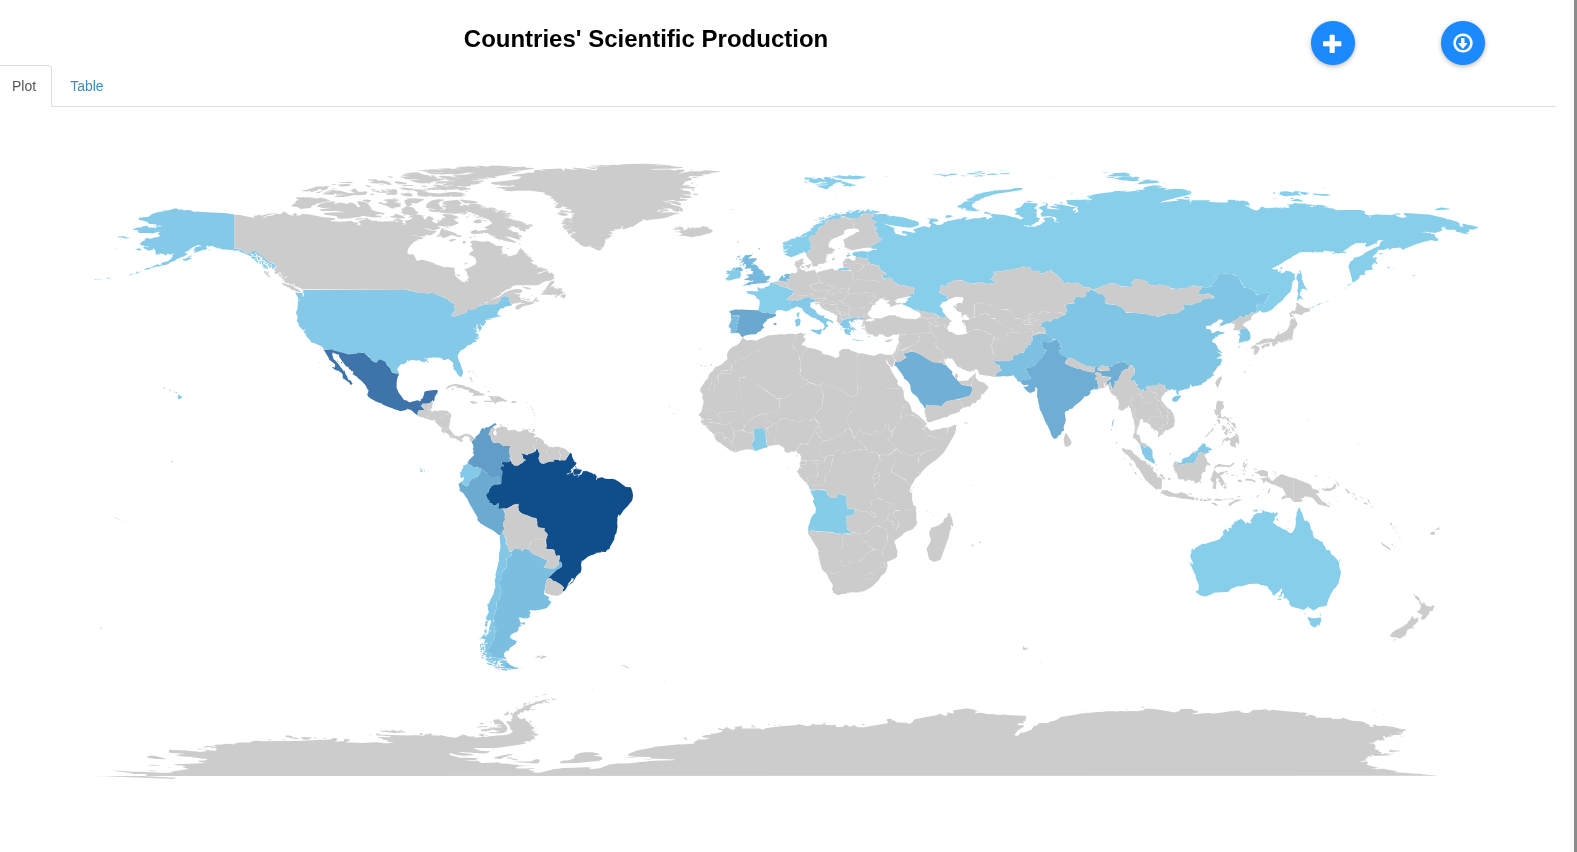
\includegraphics[width=0.8\textwidth]{Images/MapaBibliometrix.png}
    \caption{Distribución global de la producción científica sobre blockchain y gestión de infracciones.}
    \label{fig:mapa_bibliometrix}
\end{figure}

\begin{figure}[htbp]
    \centering
    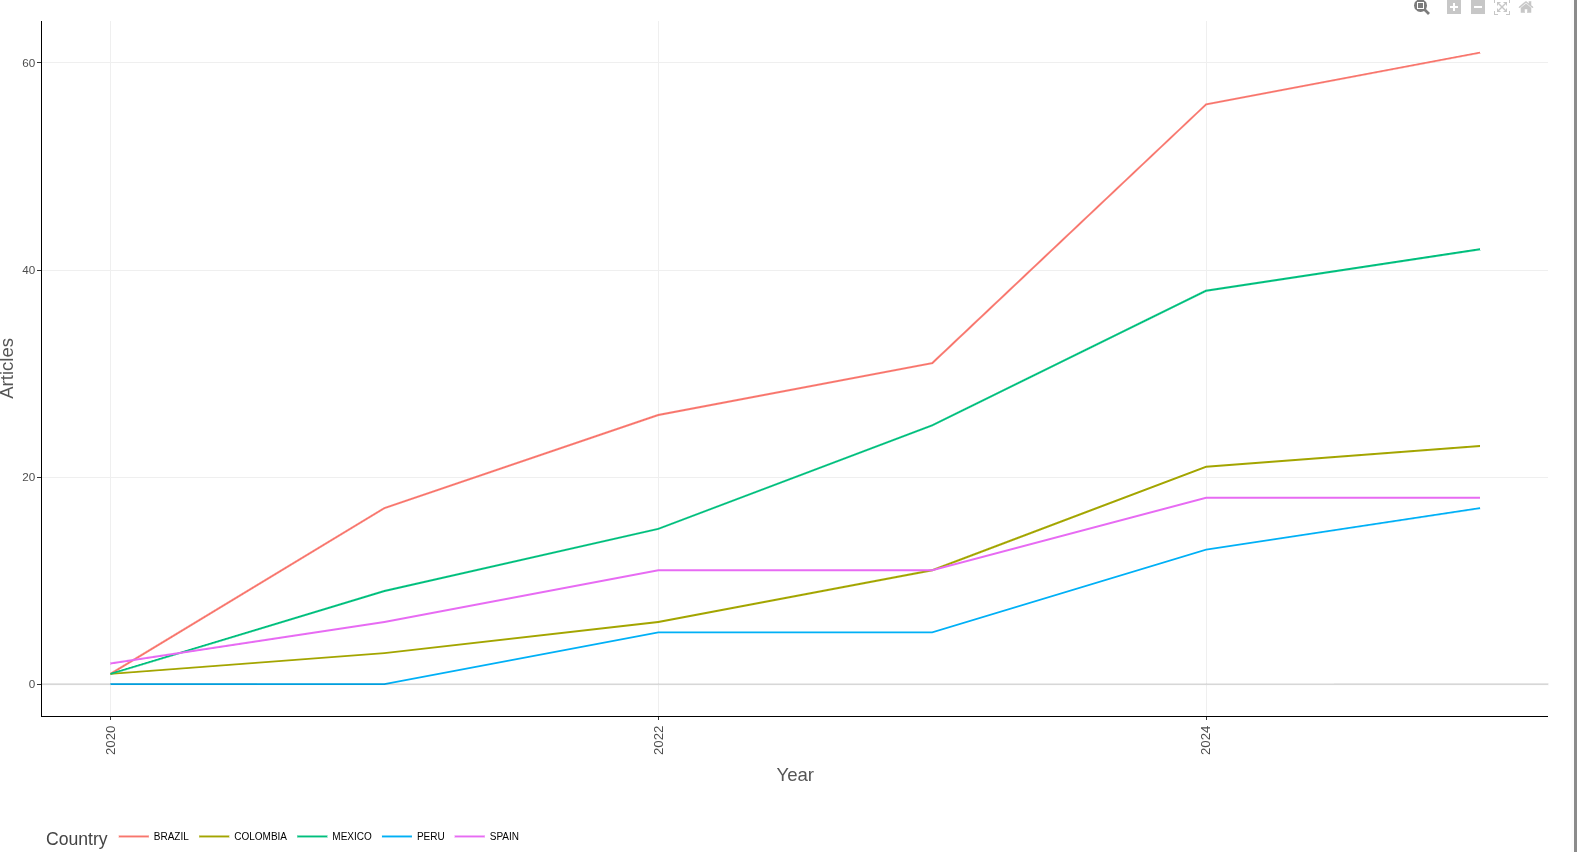
\includegraphics[width=0.8\textwidth]{Images/GraficoLineas.png}
    \caption{Evolución anual de publicaciones en los países líderes del tema (Brasil, México, Colombia, España y Perú).}
    \label{fig:grafico_lineas}
\end{figure}

\paragraph{Nube de Palabras}
La Figura~\ref{fig:nube_palabras} muestra los términos más frecuentes en la literatura analizada. Destacan conceptos como \textit{blockchain}, \textit{challenges}, \textit{management} y \textit{secure}, lo que refleja el énfasis de la comunidad académica en los retos de seguridad y gestión al aplicar tecnologías DLT en contextos gubernamentales.

\begin{figure}[htbp]
    \centering
    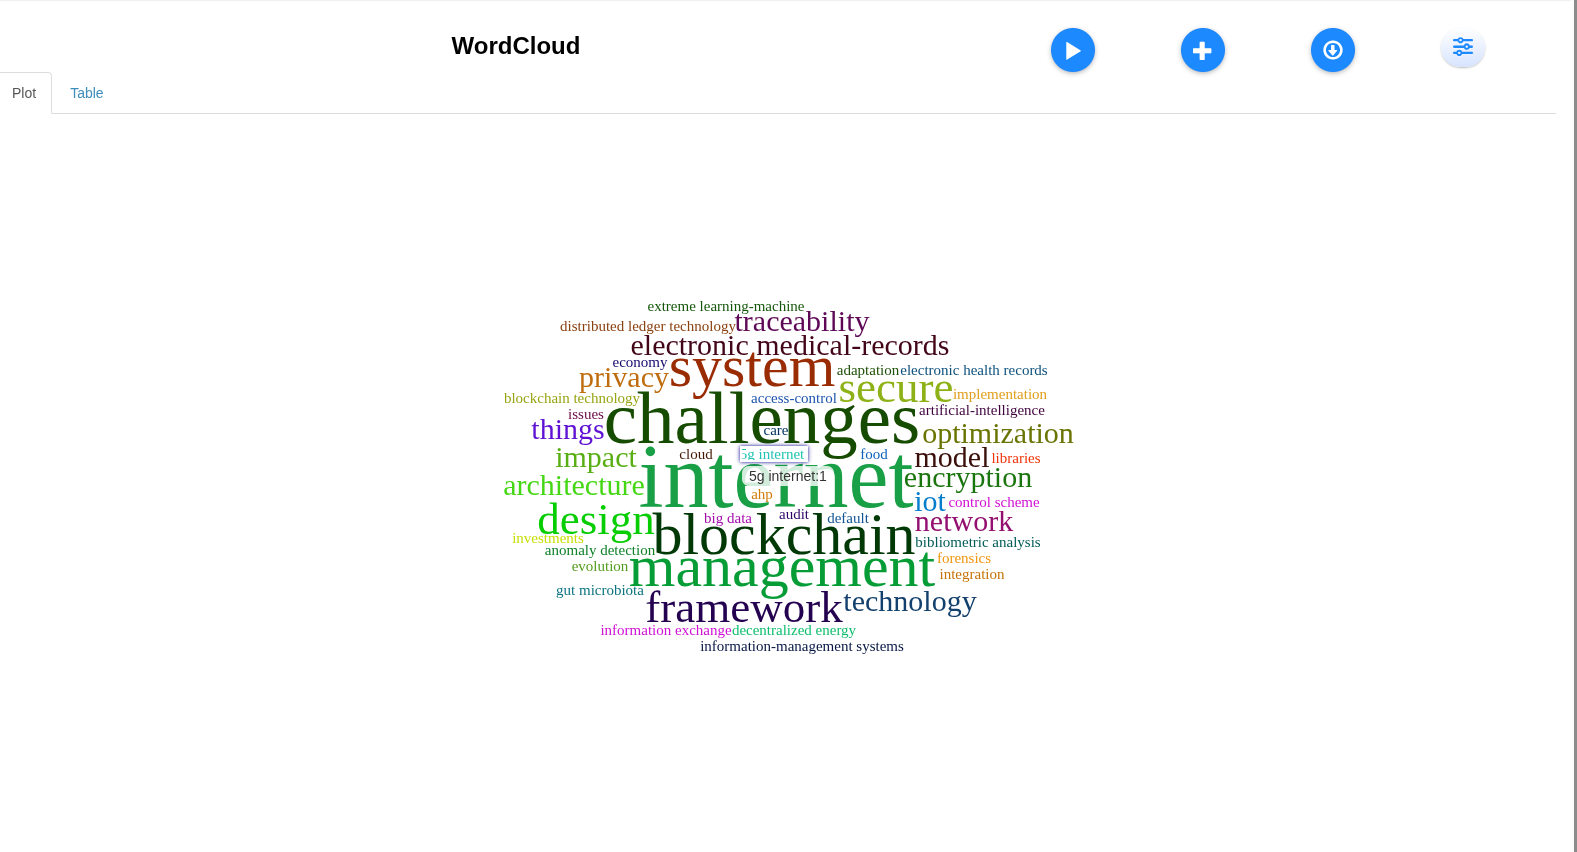
\includegraphics[width=0.8\textwidth]{Images/NubePalabras.png}
    \caption{Nube de palabras de los términos más recurrentes en la literatura sobre blockchain e infracciones.}
    \label{fig:nube_palabras}
\end{figure}
% --- Fin de figuras Bibliometrix ---